\subsection{Geräteübersicht}
Der Ballwerfer ist so konzipiert, das er aus einem fix stehenden Basismodul besteht, 
welches in der Mitte des Startbereiches positioniert wird. Die Abwurfeinheit, 
welche den Ballwurfmechanismus und die Ballzuführung beinhaltet, ist auf dem Basismodul drehend gelagert. 
Ein Schrittmotor richtet die Abwurfeinheit auf das Ziel aus. Der ganze Aufbau des Ballwurfmechanismus ist möglichst einfach gehalten. 
Er besteht hauptsächlich aus zwei Acrylglasplatten, in welcher alle mechanischen Vorrichtungen gelagert sind. 
Dadurch kann der ganze Aufbau schnell und einfach angepasst oder geändert werden. 
Die Ausrichtung des Abwurfmechanismus erfolgt durch einen Schrittmotor, welcher in der drehenden Abwurfeinheit angebracht ist. 
Dadurch kann die Bauhöhe des Ballwerfers tief gehalten werden, was einen grossen Stabilitätsvorteil bietet. 
Die Drehachse der Abwurfeinheit ist an der Spitze des Ballwerfers mit einem Bolzen angebracht. 
Somit bleibt die Abwurfposition der Tennisbälle konstant am gleichen Ort.\\
Die Tennisbälle werden durch zwei Schwungräder beschleunigt. Die Schwungräder drehen gegenläufig, 
der Tennisball wird dazwischen ausgestossen. Die Zuführung der Tennisbälle erfolgt mit einem eigens gesteuerten Förderband. 
Das Förderband muss die Bälle mit konstanter Geschwindigkeit zu den Schwungrädern transportieren, 
damit alle Tennisbälle die gleiche Startenergie aufweisen. 
Dadurch ist eine gleichmässige Wurfweite und eine hohe Reproduzierbarkeit gewährleistet. \\
\begin{figure}[h!]
		\centering
		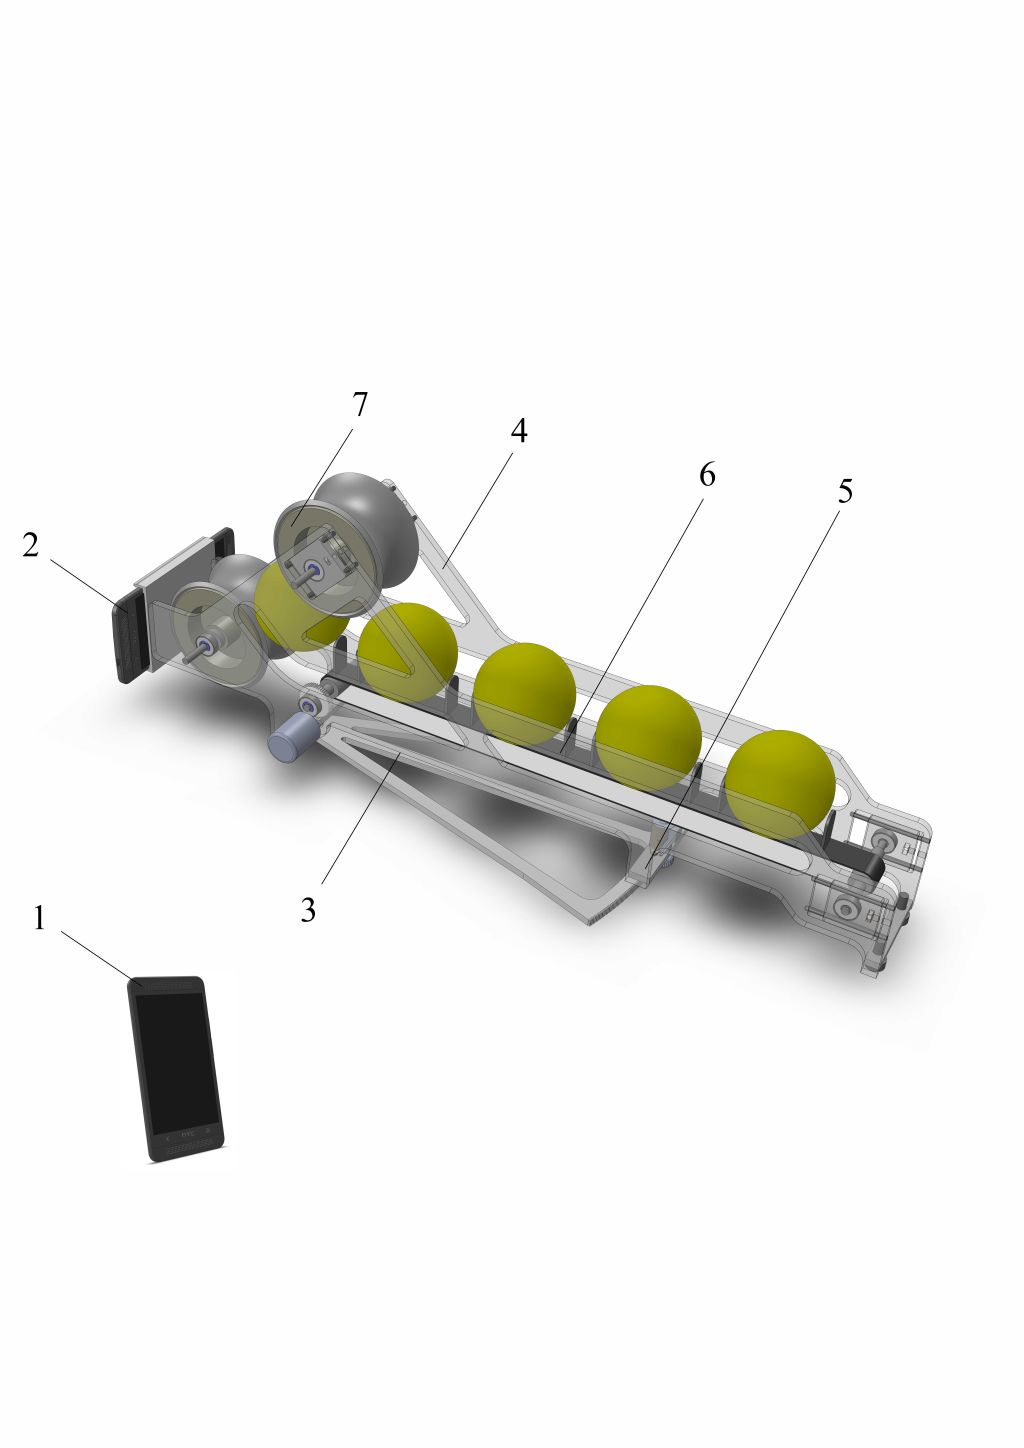
\includegraphics[width=0.95\textwidth,clip,trim=5mm 60mm 15mm 80mm] {Enddokumentation/Loesungskonzept/Bilder/Beschreibung_Komponenten-edited.jpg}
		\caption{Geräteübersicht}
		\label{fig:Geraeteuebersicht}
\end{figure}
\begin{table}[h!]
	\begin{tabular}{|c|c|p{7.5cm}|}
		\hline \textbf{Pos} & \textbf{Bezeichnung} & \textbf{Funktion} \\ 
		\hline 1 & Startgerät (Computer) & Senden des Startbefehls, Empfangen des Endbefehl, Akustische und visuelle Signalausgabe
		\\ 
		\hline 2 & Master  (Smartphone) & Empfangen des Startbefehls, Senden des Endbefehls,
		Fotografieren, Auswerten und Steuern des Controllers
		\\ 
		\hline 3 & Controller & Steuerung und Regelung der Antriebe \\ 
		\hline 4 & Gestell & Stabilisieren des Systems,
		Seitliche Führung der Bälle
		\\ 
		\hline 5 & Stelleinheit & Ausrichten des Gerätes zum Korb \\ 
		\hline 6 & Förderband & Ballförderung zu den Schwungräder \\ 
		\hline 7 & Schwungräder inkl. Antrieb & Beschleunigen der Bälle \\ 
		\hline 
	\end{tabular} 
	\centering
	\caption{Bezeichnung der Teilkomponenten}	
	\label{tab:BezTeilkomponenten}
\end{table}\\
In den folgenden Abschnitten wird nach dem zeitlichen Ablauf des Balles, die einzelnen Komponenten des Ballwerfers näher beschrieben. 